\documentclass[11pt]{article}
\usepackage[margin=1in]{geometry}
\usepackage{graphicx}
\usepackage{amsmath,amssymb}
\usepackage{booktabs}
\usepackage[colorlinks=true, citecolor=blue, linkcolor=blue, urlcolor=blue]{hyperref}
\usepackage[numbers,sort&compress]{natbib}

\title{Vibronic Coherence Across Nonadiabatic Dynamics Methods: Which Methods Reproduce Beatings, and Why?\\A Machine-Learned Hamiltonian Study}

\author{Victor M. Freixas$^{1}$ \\[2pt]
\small $^1$Department of Chemistry, University of California, Irvine \\[2pt]
\small CyberTraining 2026 project report}
\date{July 2026}

\begin{document}
\maketitle

\begin{abstract}
% TODO(1 paragraph): system, model, five dynamics, the gate finding.
The ensemble S$_1$/S$_2$ vibronic beating of a 122-atom halofluorescein
heterodimer is a stringent test of nonadiabatic molecular dynamics: it is an
ensemble coherence observable that exists only if the electronic coupling and
its geometry dependence are captured faithfully. We train a neural
quasi-diabatic Hamiltonian (NQDH) on AM1/CIS reference data and use it as a
common electronic-structure surrogate for five nonadiabatic dynamics methods
--- mean-field Ehrenfest, fewest-switches surface hopping (FSSH), surface
hopping with exact-factorization decoherence (SHXF), quantum-trajectory
surface hopping (QTSH), and full multiple spawning (FMS) --- at ensemble
scale (300 initial conditions per method), a comparison inaccessible to
direct \textit{ab initio} dynamics. The comparison isolates a single
mechanistic variable: the per-trajectory energy gate applied at transfer
events. Methods that enforce it (FSSH, SHXF, FMS in both momentum-rescaling
conventions) lose the beat; removing it (QTSH) restores the ensemble
population balance exactly, while residual stochastic hopping dephases the
coherent oscillation that only the mean-field family preserves in full.
\end{abstract}

\section{Introduction}
Photoexcited molecular aggregates funnel electronic energy through coupled
electron--nuclear motion, and one of the cleanest signatures of that coupling
is the coherent oscillation (``beating'') of excited-state populations. For a
halofluorescein AB heterodimer (122 atoms), nonadiabatic excited-state
molecular dynamics with the NEXMD package~\cite{freixas2020} revealed a
vibronic beating between the two lowest bright excitonic states $S_1$ and
$S_2$: after photoexcitation to $S_2$, the ensemble-averaged $S_2$ population
undergoes damped recurrences with a period of roughly $20$~fs before
decohering over $\sim\!90$~fs. This beating is a demanding benchmark for
nonadiabatic dynamics for three reasons. (i) It is an \emph{ensemble}
observable: individual trajectories dephase, and the beat emerges only after
averaging over a thermal ensemble of initial conditions. (ii) It is
\emph{coupling-essential}: the recurrences are driven by nuclear motion along
the nonadiabatic coupling vector (a Pechukas-type momentum kick), so freezing
the coupling destroys the beat while motion along it restores
it~\cite{freixas2023funnels}. (iii) It is \emph{coherence-sensitive}:
mean-field (Ehrenfest) dynamics reproduces it, whereas fewest-switches surface
hopping (FSSH)~\cite{tully1990}, in earlier work on this system, did not.

That last observation raises a broader, practically important question. Of the
many trajectory-based nonadiabatic dynamics methods now in wide use ---
mean-field Ehrenfest, FSSH and its decoherence-corrected
variants~\cite{minSHXF}, quantum-trajectory surface hopping
(QTSH)~\cite{martens2019qtsh,han2025qtsh}, and full multiple spawning (FMS) ---
which reproduce this vibronic beat, and what feature of each method decides the
outcome? These methods differ in how they represent electronic coherence, how
(or whether) they hop between surfaces, and how they enforce energy
conservation at a transfer event. A controlled comparison --- the same
molecule, the same electronic structure, the same initial conditions, varying
only the dynamics method --- would isolate the responsible mechanism.

Such a comparison has been out of reach for direct \emph{ab initio} dynamics.
Every method requires the electronic energies, gradients, and couplings at each
timestep; a fair ensemble comparison multiplies this by hundreds of initial
conditions and several methods, and FMS in particular spawns a growing basis of
trajectories, each carrying its own cost. The resulting thousands of
trajectory-hours of electronic-structure evaluation are prohibitive even at the
semiempirical-CI level. A fast, analytic, differentiable surrogate for the
excited-state electronic structure removes this barrier --- and, central to
this work, supplies a \emph{single common Hamiltonian} that can be handed to
independent community dynamics packages, so that differences in the results
reflect the dynamics methods and not the electronic structure.

This report demonstrates that integration. Its primary goal, as a CyberTraining
2026 software project, is to interface a trained neural quasi-diabatic
Hamiltonian (NQDH) with two established nonadiabatic dynamics codes --- the
Libra methodology package~\cite{akimov2016libra}, which supplies the
surface-hopping family and QTSH, and the pySpawn implementation of full
multiple spawning~\cite{pyspawn17} --- through a common electronic-structure
interface, and to run each method at ensemble scale ($300$ initial conditions).
As a scientific byproduct, doing so yields the controlled five-method
comparison above and localizes the beat's survival to a single mechanistic
variable: the per-trajectory energy gate applied at surface-transfer events.
The NQDH is used here purely as a fixed, pretrained electronic-structure engine;
its architecture and training are summarized for completeness
(Sec.~\ref{sec:nqdh}) and detailed separately.

\section{Methods}
\subsection{The neural quasi-diabatic Hamiltonian}
\label{sec:nqdh}
The electronic structure throughout this work is supplied by a frozen neural
quasi-diabatic Hamiltonian (NQDH). The model outputs a smooth, real, symmetric
matrix field $W(R) = D(R) + V(R)$ over nuclear configurations $R$, built on a
HIP-NN message-passing backbone~\cite{lubbers2018hipnn} that takes only atomic
numbers and Cartesian positions as input. The diagonal $D$ carries the diabatic
site energies and the off-diagonal $V$ the diabatic couplings; every adiabatic
observable follows from a single eigendecomposition $W = U\Lambda U^{T}$. The
adiabatic energies are the eigenvalues $\Lambda$, and the per-state gradients
and (scaled) nonadiabatic couplings are the diagonal and off-diagonal elements
of $M = U^{T}(\partial W/\partial R)\,U$. Because $W$ is smooth and single-valued
while the couplings diverge only through the eigendecomposition, propagating in
the diabatic representation avoids the $1/\Delta E$ singularity of the adiabatic
coupling at the $S_1/S_2$ near-degeneracy (Sec.~\ref{sec:dynamics}).

The model was trained on AM1/CIS reference data (the ground and first two
excited states) for the heterodimer: geometries sampled from ground-state
Langevin trajectories and labeled with NEXMD single-point
calculations~\cite{nexmd2020} providing energies, gradients, and transition
densities. The ground state is treated as decoupled --- its off-diagonal
couplings are structural zeros --- so only the $S_1$--$S_2$ block is dynamically
active. The specific frozen model used here (denoted v12a) reaches held-out
mean absolute errors of $25$ and $27$~meV on the $S_0$--$S_1$ and $S_0$--$S_2$
excitation energies and $33$~meV on the $S_1$--$S_2$ dynamics gap
(Fig.~\ref{fig:parity}). Its development --- the active-learning and loss-design
choices behind those numbers --- is beyond the scope of this software-focused
report and is described elsewhere. For all dynamics below the model is fixed: it
functions purely as a drop-in electronic-structure engine returning $W(R)$ and
$\partial W/\partial R$ in atomic units.

\begin{figure}[t]
  \centering
  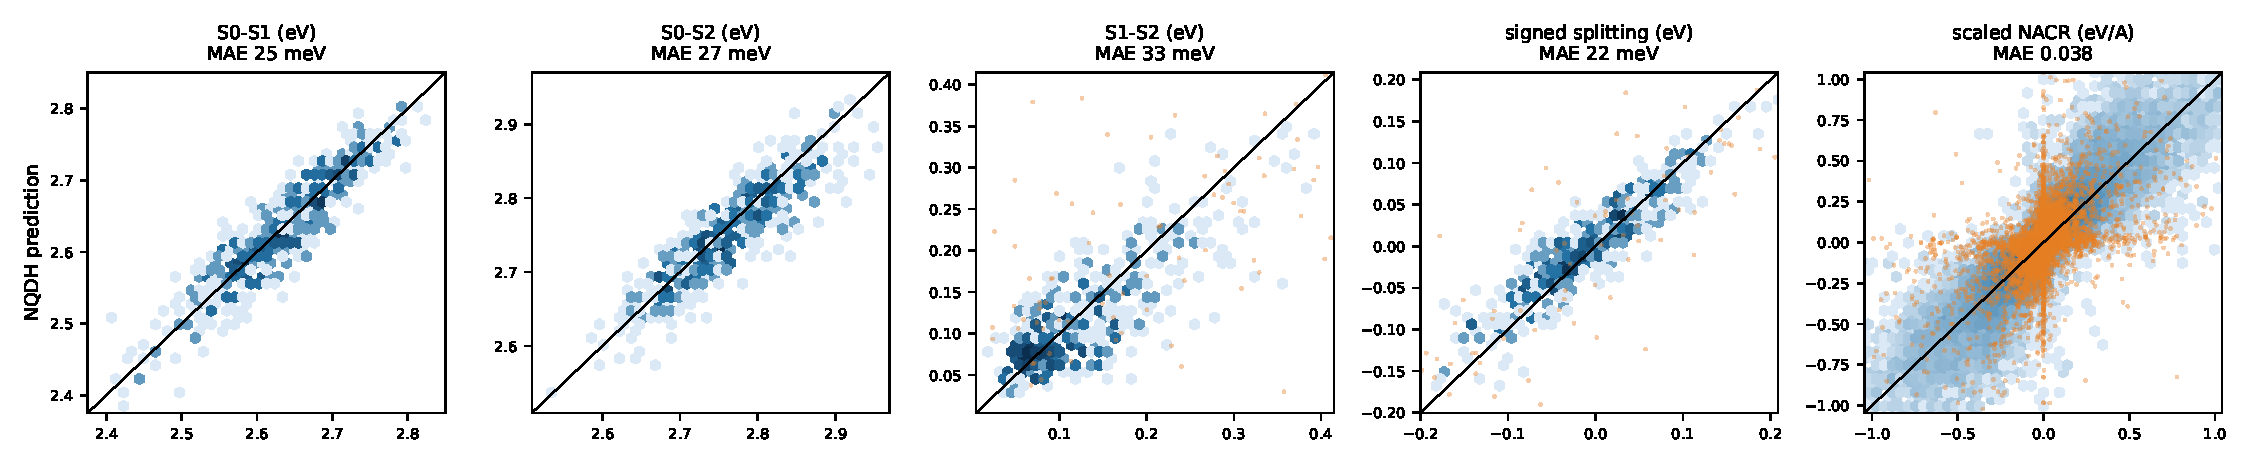
\includegraphics[width=\linewidth]{figures/F2_model_parity/figure.pdf}
  \caption{Model card: held-out parity of the frozen NQDH (v12a) against
  NEXMD references. Left to right: the two absorption gaps, the dynamics
  gap, the signed diabatic splitting, and the scaled-NACR components.
  Blue density: thermal test set; orange: displaced (post-excitation)
  geometries. \textit{TODO: final stats in caption.}}
  \label{fig:parity}
\end{figure}

\subsection{Dynamics}
\label{sec:dynamics}
All dynamics methods consume the identical electronic structure through a thin
provider: given atomic numbers and Cartesian coordinates (bohr), it returns the
diabatic Hamiltonian $W$ (Hartree) and its Cartesian derivatives
$\partial W/\partial R$ (Hartree/bohr) by automatic differentiation of the
frozen model. From these, a single eigendecomposition per geometry yields the
adiabatic energies $E_i$, the per-state forces $-(U^{T}\partial W/\partial R\,U)_{ii}$,
and the derivative couplings $(U^{T}\partial W/\partial R\,U)_{ij}/(E_j-E_i)$.
Three engines are driven from this common interface: a reference diabatic
Ehrenfest integrator, the Libra surface-hopping family, and pySpawn full
multiple spawning.

\subsubsection{Reference diabatic Ehrenfest}
Mean-field Ehrenfest dynamics propagates the nuclei under the force
$F = -\mathrm{Tr}(\rho\,\partial W/\partial R)$, with $\rho$ the electronic
density matrix, while the electronic amplitudes evolve as
$i\hbar\,\dot{c} = W c$ directly in the diabatic basis; adiabatic populations
are recovered by diagonalizing $W$ along the trajectory. We implemented this in
a short, self-contained NumPy integrator (velocity-Verlet nuclei,
exponential-midpoint electronic substepping) that serves both as the physical
reference and as a validation target for the software interface: propagated from
an identical initial condition, our engine and Libra's Ehrenfest agree on the
adiabatic populations to better than $10^{-5}$ over the full $194$~fs window,
confirming that the two codes consume the model consistently.

\subsubsection{Libra interface: surface hopping and QTSH}
Libra's trajectory-dynamics driver (\texttt{tsh.generic\_recipe}) expects the
electronic structure as a \texttt{compute\_model} callback in its
model-Hamiltonian convention. We provide an adapter that, on each call,
evaluates the provider at the requested geometry and packs the result into
Libra objects: the diabatic Hamiltonian \texttt{ham\_dia} (a $K\times K$
\texttt{CMATRIX}), an identity overlap \texttt{ovlp\_dia} (the diabats are
orthonormal), the $K\times K$ derivative matrices \texttt{d1ham\_dia} (one per
nuclear degree of freedom), and zero derivative-coupling matrices
\texttt{dc1\_dia} (strict diabats carry no derivative coupling). The adapter is
molecule-agnostic; all model-specific work stays in the provider.

Within this single interface the methods differ only in Libra's hop-acceptance,
momentum-rescaling, and decoherence parameters --- the controlled variables of
the comparison (Table~\ref{tab:presets}). FSSH accepts a stochastic hop only if
the kinetic energy along the derivative-coupling direction can pay the energy
gap (\texttt{hop\_acceptance\_algo}~$=20$) and rescales the momentum along that
direction (\texttt{momenta\_rescaling\_algo}~$=201$); a rejected hop is
``frustrated.'' SHXF adds independent-trajectory exact-factorization decoherence
(\texttt{decoherence\_algo}~$=5$), with auxiliary-wavepacket widths set from
standard frozen-Gaussian exponents, while retaining the FSSH energy gate. QTSH
instead accepts every proposed hop (\texttt{hop\_acceptance\_algo}~$=0$) and
applies no momentum jump (\texttt{momenta\_rescaling\_algo}~$=0$); energy is
conserved over the ensemble, not per trajectory, through a coherence-weighted
nonclassical force (\texttt{use\_qtsh}~$=1$). Thus FSSH and SHXF impose the
per-trajectory energy gate whereas QTSH removes it --- the single distinction on
which the results turn.

\begin{table}[t]
  \centering
  \small
  \begin{tabular}{lccc}
    \toprule
    parameter & FSSH & SHXF & QTSH \\
    \midrule
    \texttt{hop\_acceptance\_algo}   & 20  & 20  & 0 \\
    \texttt{momenta\_rescaling\_algo}& 201 & 201 & 0 \\
    \texttt{decoherence\_algo}       & --- & 5   & --- \\
    \texttt{use\_qtsh}               & 0   & 0   & 1 \\
    per-trajectory energy gate       & yes & yes & no \\
    \bottomrule
  \end{tabular}
  \caption{Libra \texttt{dyn\_params} presets driven through the common NQDH
  \texttt{compute\_model} adapter. The three methods differ only in these
  hop/rescale/decoherence knobs; all other settings (representation, time
  overlap, substepping) are identical.}
  \label{tab:presets}
\end{table}

\subsubsection{pySpawn interface: full multiple spawning}
pySpawn builds its electronic-structure method by grafting a ``potential''
module onto its trajectory class. We supply a module that, at each geometry,
sets the adiabatic energies (eigenvalues of $W$), the per-state forces, and ---
central to the interface --- the electronic wavefunctions as the eigenvector
rows $U^{T}$ in the fixed diabatic basis. pySpawn's nearest-previous-%
interpolation time-derivative coupling then consumes the overlap of successive
wavefunctions, which for our fixed-basis eigenvectors is exactly
$U(t)^{T}U(t{+}\Delta t)$; a clamp guards the rare round-off case
$|\text{overlap}| = 1+\varepsilon$ that would otherwise return \texttt{NaN}.

Because a spawn is followed by an energy-conserving momentum adjustment of the
child trajectory --- the FMS analog of the surface-hopping gate --- we expose it
as a controlled variable. The stock behavior rescales the child momentum by a
scalar along the full velocity vector; we additionally implement an override
that adjusts the momentum along the $S_1$--$S_2$ derivative-coupling direction
(the physical Pechukas direction), solving the same energy-conservation
condition for the component along that direction. Either mode aborts the spawn
(``frustrated'') when insufficient energy is available. Every spawn attempt is
logged with its time and outcome (accepted or frustrated), providing the raw
data for the timing analysis in Sec.~\ref{sec:results}.

\subsubsection{Ensemble protocol and execution}
The $300$ initial conditions are drawn from the ground-state thermal ensemble
(positions and velocities from the Langevin trajectories, corresponding to
$300$~K), each photoexcited vertically to the bright $S_2$ state. Ehrenfest and
Libra surface-hopping trajectories are propagated for $2000$ steps of
$\Delta t = 4$~a.u.\ ($\approx\!194$~fs), the hopping methods using two
stochastic replicas per initial condition. Full multiple spawning is
substantially more expensive --- its cost grows with the number of spawned basis
functions --- and is propagated to $1650$~a.u.\ ($\approx\!40$~fs, covering the
first recurrences) for each initial condition in both momentum-rescaling modes.
The Libra ensembles ran on a single GPU; the FMS ensembles ran as SLURM job
arrays on the UCI Green Planet cluster, one CPU task per (initial condition,
rescale mode).

\section{Results}
\label{sec:results}
\subsection{The learned Hamiltonian reproduces the vibronic beat}
\begin{figure}[t]
  \centering
  
\includegraphics[width=0.8\linewidth]{figures/F3_ensemble_beat/figure.pdf}
  \caption{The S$_1$/S$_2$ vibronic beat from 300-trajectory diabatic
  Ehrenfest ensembles on the frozen NQDH: recurrences every $\sim$18\,fs
  decohering by $\sim$90\,fs, in agreement with the reference NEXMD
  phenomenology. Inset: progression across model generations.
  \textit{TODO: annotate recurrence times.}}
  \label{fig:beat}
\end{figure}
% TODO: text.

\subsection{The energy gate decides survival of the beat}
% FIGURE F4 (single-IC five dynamics) -- data returns with the desktop:
% 
\includegraphics{figures/F4_five_dynamics_single_ic/figure.pdf}
% FIGURE F5 (300-IC ensemble verdict incl. FMS) -- FMS ensemble in flight:
% 
\includegraphics{figures/F5_ensemble_gate_verdict/figure.pdf}
% TODO: text + Table~\ref{tab:scoreboard}.

\subsection{When the gate closes: timing of frustrated events}
% FIGURE F6 (frustration-time histogram vs recurrence windows) -- from the
% FMS ensemble event logs; prediction registered before the data: frustrated
% events cluster at the seam-return windows.

\section{Analysis}
% TODO: the 2x2 (gate x population flow); the upward-transfer energy-gate
% mechanism; QTSH stochastic dephasing (level right, oscillation washed);
% consistency with the AIMC / reduced-dimensional wavepacket record.

\section{Discussion}
% TODO: implications for method choice when the observable is a coherence;
% why ~40 meV pointwise gap errors still carry the physics (differential
% accuracy; the observable selects its error projections); limitations:
% far-region model softness, ntraj replica caveat, Ehrenfest as
% reference-not-truth, classical nuclei for deeply quantum modes
% (hbar*omega ~ 9-12 kT).

\section{Proposed directions}
% TODO: QTAG on the learned branching plane (potential-evaluation wall
% removed; traveling-basis problem characterized -- 7-attempt ledger);
% MQCXF configuration question; MCTDH on the analytically extracted
% vibronic model; HEOM/TENSO system-bath route; the derivative tower.

\section{Conclusions}
% TODO.

\section*{Code and data availability}
All code, the frozen model, initial conditions, and per-figure data/scripts
are available in this repository
(\url{https://github.com/vmfreixas/nqdh-beating-demo}).

\section*{Acknowledgments}
% TODO: CyberTraining 2026 (NSF award #), Akimov group / Libra, pySpawn,
% Green Planet cluster (UCI).

\bibliographystyle{unsrtnat}
\bibliography{refs}

\end{document}
